\begin{frame}
 \frametitle{The \Qweak\ Experiment}
 \begin{block}{Current mode}
  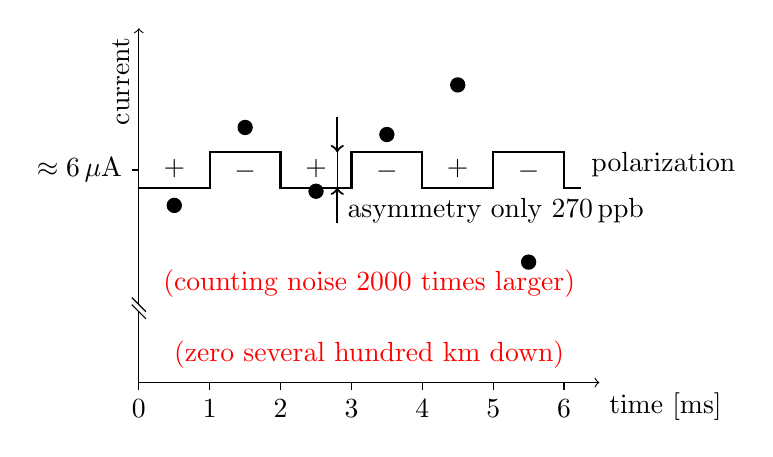
\begin{tikzpicture}[scale=0.9]
   % Time axis and ticks
   \draw[->] (0,0) -- (6.5,0) node[below right]{time [ms]};
   \node<2->[red] at (3.25,0.4) {(zero several hundred km down)};
   \foreach \x/\y in {0/4.5,1/4.5,2/4.5,3/4.5,4/4.5,5/4.5,6/4.5}
    \draw (\x,0) -- (\x,-0.1) node[below] {$\x$};
   % Current axis, interrupt and ticks
   \draw (0,0) -- (0,1);
   \draw (0.1,0.9) -- (-0.1,1.1);
   \draw (0.1,1.0) -- (-0.1,1.2);
   \draw[->] (0,1.1) -- (0,5) node[above left,rotate=90]{current};
   \draw (0,3.) -- (-0.1,3.0) node[left] {$\approx 6\,\mu$A};
   % Helicity windows
   \draw[thick]
    (0,2.75) -- node[above]{$+$} (1,2.75) --
    (1,3.25) -- node[below]{$-$} (2,3.25) --
    (2,2.75) -- node[above]{$+$} (3,2.75) --
    (3,3.25) -- node[below]{$-$} (4,3.25) --
    (4,2.75) -- node[above]{$+$} (5,2.75) --
    (5,3.25) -- node[below]{$-$} (6,3.25) --
    (6,2.75) -- (6.24,2.75) node[above right]{polarization};
   % Asymmetry
   \draw[thick,->] (2.8,3.75) -- (2.8,3.25);
   \draw[thin]     (2.8,3.25) -- (2.8,2.75);
   \draw[thick,->] (2.8,2.25) -- (2.8,2.75) node[below right]{asymmetry only 270\,ppb};
    % Data points
    \foreach \x/\y in {0/2.5,1/3.6,2/2.7,3/3.5,4/4.2,5/1.7}
     \draw<3->[fill] (0.5+\x,\y) circle (0.1);
   \node<3->[red] at (3.25,1.4) {(counting noise 2000 times larger)};
  \end{tikzpicture}
 \end{block}
 \begin{itemize}
  \item Collect many polarization windows: \alert{2 year long} experiment
  \item Ensure that scatter is uncorrelated and perfectly Gaussian
 \end{itemize}
\end{frame}
